
\usetikzlibrary{arrows}

\ifnumequal{\value{rolldice}}{0}{
  \renewcommand{\va}{A}
  \renewcommand{\vb}{B}
  \renewcommand{\vc}{C}
  \renewcommand{\vd}{D}
}{
  \ifnumequal{\value{rolldice}}{1}{
    \renewcommand{\va}{L}
    \renewcommand{\vb}{M}
    \renewcommand{\vc}{N}
    \renewcommand{\vd}{O}
  }{
    \ifnumequal{\value{rolldice}}{2}{
      \renewcommand{\va}{P}
      \renewcommand{\vb}{Q}
      \renewcommand{\vc}{R}
      \renewcommand{\vd}{S}
    }{
      \renewcommand{\va}{H}
      \renewcommand{\vb}{I}
      \renewcommand{\vc}{J}
      \renewcommand{\vd}{K}
    }
  }
}

\question Below is a schedule of four transactions ($T_1$, $T_2$, 
$T_3$, $T_4$) with their events listed in chronological order. 
Assume that when a transactions requests -\\
\watchout
\begin{tabular}{ll}
an Exclusive lock $X(?)$ &$\Rightarrow$ it performs a \texttt{read} followed by a \texttt{write} \\
a  Shared lock $S(?)$    &$\Rightarrow$ it performs a \texttt{read} \\
an Unlock $U(?)$         &$\Rightarrow$ it releases the \texttt{lock} \\
\end{tabular}
\\
\begin{tabular}{|c|c|c|c|c||c|c|c|c|c|}
  \hline
  Event & $T_1$ & $T_2$ & $T_3$ & $T_4$ &Event & $T_1$ & $T_2$ & $T_3$ & $T_4$ \\
  \hline
  $1$   & -       & $S(\va)$& -       & -       &$13$  & -       & -       & $U(\vb)$& -       \\
  $2$   & -       & -       & -       & $S(\va)$&$14$  & $X(\vb)$& -       & -       & -       \\
  $3$   & -       & $X(\vb)$& -       & -       &$15$  & -       & -       & $U(\vd)$& -       \\
  $4$   & -       & $S(\vc)$& -       & -       &$16$  & -       & -       & $U(\va)$& -       \\
  $5$   & $S(\va)$& -       & -       & -       &$17$  & $U(\vb)$& -       & -       & -       \\
  $6$   & -       & -       & -       & $U(\va)$&$18$  & -       & -       & -       & $S(\vd)$\\
  $7$   & -       & -       & $S(\va)$& -       &$19$  & $U(\vc)$& -       & -       & -       \\
  $8$   & -       & $U(\vb)$& -       & -       &$20$  & -       & -       & -       & $S(\vc)$\\
  $9$   & -       & -       & $S(\vb)$& -       &$21$  & $U(\va)$& -       & -       & -       \\
  $10$  & -       & -       & $X(\vd)$& -       &$22$  & -       & $U(\va)$& -       & -       \\
  $11$  & -       & $U(\vc)$& -       & -       &$23$  & -       & -       & -       & $U(\vd)$\\
  $12$  & $X(\vc)$& -       & -       & -       &$24$  & -       & -       & -       & $U(\vc)$\\
  \hline
\end{tabular}
\\

\begin{parts}
  \part[3] Determine whether the schedule is serializable 
  \textit{(yes or no)} and justify your answer.

  \begin{solution}[\fullpage]
    To determine serializability, we must examine each request for
    an Exclusive lock in relation with the reads before and after
    that resource.\\
    Consider resource $\va$:
    \begin{align}
      \text{No exclusive locks requested therefore no constraints} \nonumber
    \end{align}     
    Consider resource $\vb$:
    \begin{align}
      T_2(E=3\,\texttt{write}) &\rightarrow T_3(E=9\,\texttt{read}) \\
      T_2(E=3\,\texttt{write}) &\rightarrow T_1(E=14\,\texttt{read,write}) \\
      T_3(E=9\,\texttt{read})  &\rightarrow T_1(E=14\,\texttt{read,write}) 
    \end{align}
    Consider resource $\vc$:
    \begin{align}
      T_2(E=4\,\texttt{read})        &\rightarrow T_1 (E=12\,\texttt{read,write}) \\
      T_1(E=12\,\texttt{read,write}) &\rightarrow T_4 (E=20\,\texttt{read}) \\
    \end{align}
    Consider resource $\vd$:
    \begin{align}
      T_3(E=10\,\texttt{read,write}) &\rightarrow T_4 (E=18\,\texttt{read})
    \end{align}
    Given the constraints above, precedence graph would be as shown\\
    \begin{center}
    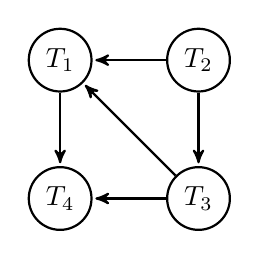
\begin{tikzpicture}[->,>=stealth',shorten >=1pt,auto,node distance=50pt, thick,main node/.style={circle,draw}]
      \node[main node] (1) {$T_1$};
      \node[main node] (2) [ right of=1] {$T_2$};
      \node[main node] (3) [ below of=2] {$T_3$};
      \node[main node] (4) [ below of=1] {$T_4$};
      
      \path[every node/.style={font=\sffamily\small}]
        (1) edge node [left] {} (4)
        (2) edge node [right] {} (1)
        (2) edge node [right] {} (3)
        (3) edge node [right] {} (4)
        (3) edge node [left] {} (1);
      
    \end{tikzpicture}
    \end{center}
    Since the graph does not contain any cycles, the schedule is serializable.
  \end{solution}

  \part[3] If it is serializable, provide an equivalent serial schedule.
  Justify your answer by showing intermediary steps. If it is not 
  serializable, show how \texttt{Two Phase Locking} would have prevented 
  the schedule.

  \begin{solution}[\halfpage]
    One equivalent serial schedule is:
    \begin{align}
      T_2 \longrightarrow T_3 \longrightarrow T_1 \longrightarrow T_4
    \end{align}
  \end{solution}

  \part[3] Does the schedule follow \texttt{Two-Phase Locking} protocol?
  Answer \textit{yes or no} and justify your answer.

  \begin{solution}[\halfpage]
    For a schedule to follow \texttt{Two-Phase Locking} protocol, it must
    have a clear separation between \textit{acquisition} phase, where it 
    acquires locks followed and \textit{release} phase where it releases 
    locks.\\
    In the given schedule $T_4$ acquires locks on $\vd(E=18)$ and then again
    on $\vc(E=20)$ after it releases it's lock on $\va(E=6)$. Therefore it 
    does not follow the \texttt{Two-Phase Locking} protocol.
  \end{solution}

\end{parts}

